\documentclass{llncs}

\usepackage{hyperref}
\usepackage{graphicx}
\usepackage{listings}

\begin{document}

\title{A linked open data architecture for contemporary historical archives}  
\author{Alexandre Rademaker\inst{1} 
  \and Suemi Higuchi\inst{2}
  \and D\'ario Augusto Borges Oliveira\inst{2}}
\institute{IBM Research and FGV/EMAp \and FGV/CPDOC}
\maketitle

\begin{abstract}
  This paper presents an architecture for historical archives
  maintenance based on Open Linked Data technologies and open source
  distributed development model and tools. The proposed architecture
  is being implemented for the archives of the Center for Teaching and
  Research in the Social Sciences and Contemporary History of Brazil
  (CPDOC) from Getulio Vargas Foundation (FGV).
\end{abstract}

\section{Introduction}\label{sec:intro}

% 1. the use of open/linked data vs. relational data
% 2. embracing the open source development model for data maintainnability
% 3. CPDOC ownership versus curatorship of the datasets
%
% The Center for Research and Documentation of Contemporary History of
% Brazil (CPDOC) of Getulio Vargas Foundation (FGV) is an institution
% dedicated to study and preserve content from the Brazilian
% contemporary history.  CPDOC holds rich collections of personal
% archives, interviews and different audiovisual sources very
% important for understanding part of Brazilian memory. During the
% 70's and 80's, CPDOC team developed its own methodology for
% organizing and indexing documents, recognized as innovative by
% leading educational and research institutions. However, new
% technologies and trends for data sharing and interoperability of
% collections pose a challenge to CPDOC to remain innovative in its
% mission of efficiently dealing with historical data. It is time to
% adjust CPDOC methodology to new paradigms.

The Center for Teaching and Research in the Social Sciences and
Contemporary History of Brazil (CPDOC) was created in 1973 and became
an important historical research institute, housing a major collection
of personal archives, oral histories and audiovisual sources that
document the country memory. It is part of Getulio Vargas Foundation
(FGV), a prestigious Brazilian research and higher education
institution founded in 1944, considered by Foreign Policy Magazine to
be a top-5 ``policymaker think-tank'' worldwide \cite{think-tank}.

Thanks to the donation of the personal archives of President Getulio
Vargas and other brazilian figures who had been prominent from the
1930s onward, CPDOC started to develop its own methodology for
organizing and indexing documents, and by the end of the 1970s, it was
already recognized as a reference among research and historic
documentation centers. In 1975, the institute launched its Oral
History Program (PHO), which involved the execution and recording of
interviews with people who participated in major events in Brazilian
history. In 1984, CPDOC published the Brazilian
Historical-Biographical Dictionary (DHBB) \cite{dhbb}, a regularly
updated reference resource that documents the contemporary history of
the country. In the late 1990s, CPDOC was recognized as center of
excellence by the Support Program for Centers of Excellence (Pronex)
of the Brazilian Ministry of Science and Technology
% , after a dispute with several other institutions in the area of
% humanities.
% In the last ten years it started offering graduate and undergraduate
% courses in Social Sciences and History, receiving maximum score in the
% latest assessment by the Brazilian Ministry of Education.

CPDOC is a vibrant and diverse intellectual community of scholars,
technicians and students, and has placed increasing emphasis on
applied research in recent years, working in collaborative projects
with other schools and institutes, aiming at extend the availability
and scope of the valuable records it holds. 

% However, trends for data sharing and interoperability of digital
% collections pose a challenge to the institute to remain innovative in
% its mission of efficiently dealing with historical data. It is time to
% adjust CPDOC methodology to new paradigms.

This year, when completes 40 years of existence, CPDOC will have the
support of the Brazilian Ministry of Culture (MinC), which is going to
provide a fund of R\$ 2.7 million to finance the project
``Dissemination and Preservation of Historical Documents'' wich has
the following main goals: (1) digitilizing a significative amount of
textual, iconographic and audiovisual documents; (2) updating the
dictionary DHBB; and (3) prospecting innovative technologies that
enable new uses for CPDOCs collections.

The advances in technology offer new modes of dealing with digital
contents; the number of approaches increases as new technological
tools are developed.  CPDOC is committed to offering swift access to
its archives and is working toward making all data available in a more
intelligent/semantic way, in the near future. In collaboration with
the FGV School of Applied Mathematics (EMAp), CPDOC is working on a
project that aims to enhance access to documents and historical
records by means of data-mining tools, semantic technologis and signal
processing. At the moment, two applications are being explored: (1)
face detection and identification in photographs, and (2) voice
recognition in the sound and audiovisual archives of oral history
interviews. Soon it will be easier to identify people in photographs,
and then search for them in the archives after they have been
identified. Additionally, voice recognition will help locate specific
words and phrases in audiovisual sources based on their alignment with
transcription -- a tool that is well-developed for English recordings
but not for Portuguese. Both of these processes involve machine
learning and natural language processing, since the computer must be
taught to recognize and identify faces and words.

%The progressive conversion of the analog to digital formats has
%reached a limit in which every product of human intellectual activity
%is born digital or soon will be available in some electronic
%format. The predominance of this modality brings changes not only in
%the way we elaborate and express knowledge, but also in how we
%acquire, store, share and use it.
   
Also, CPDOC wants that your data constitute a large knowledge base
accessible by the standards of semantic computing. Despite having
become a reference in the field of organization of collections, CPDOC
currently do not adopt any metadata standards nor any open data model
for them. Trends for data sharing and interoperability of digital
collections pose a challenge to the institution to remain innovative
in its mission of providing efficiently historical data. It is time to
adjust CPDOC's methodology to new paradigms.
   
% CPDOC is committed to offering swift access to its archival materials
% and is working toward making all data available in a more
% intelligent/semantic way, in the near future. This process includes
% engaging with the public and using innovative, new techniques in
% managing the archives. Currently these archives are not following any
% metadata standards nor any open data model that could facilitate
% interoperability between information systems.

% Metadata or meta information can be defined as "data that describes
% data '. Libraries, museums and documentation centers make use of
% metadata for purposes of cataloging and describing objects that
% integrate their collections, with a focus on access to
% information. Initiatives such as Dublin Core \cite{dc}, Encoded
% Archival Description (EAD) \cite{ead} and Text Encoding Initiative
% (TEI) \cite{tei} are some examples of metadata models developed for
% digital libraries and represent a major advance in the matter of
% interoperability and information exchange between
% repositories. Besides, some studies shows that the use of
% ontology-based metadata can be a promising way. In a case study,
% Weinstein \cite{Weinstein98ontology} carried out the conversion of a
% bibliographic catalog encoded in MARC format for a model of
% ontology, obtaining a knowledge base with descriptions much richer
% and expressive. This implies that the queries are mapped to the
% conceptual structure of the ontology, ie, the relationships embedded
% in it and not only by attributes values.
      
This article introduces a research project that reflects a change in
the way CPDOC wants to deal with archives maintenance and
difusion. The project is an ongoing initiative to build a model of
data organization and storage that ensures easy access,
interoperability and reuse by service providers. The project proposal
is inspired by: (1) Open Linked Data Initiative principles \cite{odi};
(2) distributed open source development model and tools for easy and
collaborative data maintenance; (3) a growing importance of data
curation concepts and practices for online digital archives management
and long-term preservation.
   
The project started with an initiative of creating a linked open data
version of CPDOC's archives and a prototype of a simple and intuitive
web interface for browsing and searching the archives. The uses of
Linked Open Data concept are conformed to the three laws first
published by David Eaves~\cite{3-law} and now widely accepted: (1) If
it can't be spidered or indexed, it doesn't exist; (2) If it isn't
available in open and machine readable format, it can't engage; and
(3) If a legal framework doesn't allow it to be repurposed, it doesn't
empower.
  
Our ideas are aligned with those proposed by the Semantic Web
community, it is an effort to build a global network of interconnected
open data. 

% This conception improves dramatically the possibility of discovering
% new knowledge as a straightforward consequence of adopting open
% standard formats with ensured accessibility. 
Among the initiatives of this project we emphasize the construction of
a RDF~\cite{rdf-primer} data from data originally stored in a
relational database, the construction of an OWL~\cite{owl} ontology to
allow the proper represent the CPDOC domain.
% definition and interoperability of data in CPDOC. 
The proposal also aims of making the whole RDF data available for
download following DBPedia approach~\cite{dbpedia}. Brazil has a good
supply of public data available for free, but very few are in open
format, under the semantic web accepted standards. Examples in this
direction are the Governo Aberto SP~\cite{gasp}, the
LeXML~\cite{lexml} and the SNIIC project~\footnote{Sistema Nacional de
  Informações e Indicadores Sociais,
  \url{http://culturadigital.br/sniic/}.}.
   
This paper reflects a real effort grounded in research experience to
maintain CPDOC as a reference institution in the field of historic
preservation and documentation in Brazil.

% CPDOC has observed the evolution of our society by means of the
% irreversible process of globalization and informatization. This
% process has evolved together with new ways of learning and teaching,
% acquiring, storing and using data that allow people to use
% information as easily accessible knowledge. In this scenario, FGV, a
% youthful and nimble institution, remains aware of its precursor role
% of dealing with knowledge using new technologies.

% CPDOC is aware of that the process of digitalization and
% globalization of our society requires new methods of learning,
% teaching, acquiring, storing and using informations as so to
% transform it into actionable knowledge. In this scenario, FGV is
% uniquely positioned to lead in this new reality, being a youthful
% and nimble knowledge-based institution.

% Even though it is about the same universe of discourse -- the
% contemporary history of Brazil -- three different information
% systems were built to store the different types of documents.

% One of the greatest CPDOC's concerns is to make their archives
% widely visible online and interoperable with other digital
% archives. Currently these archives are not following any standard
% open data model, and queries to collections are limited to what
% systems in CPDOC offer, which is not much. The data is not
% accessible from outside and service providers cannot use CPDOC
% collections in their services, pontentially spreading the
% institution's audience.

% In the current state, CPDOC main concern is that its archives are
% not following any standard open data model. This scenario does not
% help to make the CPDOC's archives widely visible online and
% interoperable with other digital archives. Thus, queries to CPDOC's
% collections are limited to what CPDOC systems can offer and service
% providers could not use CPDOC collections in their services that
% could potentially reach a wide audience.

% We believe that CPDOC must review its methodology for digital data
% maintenance, storage, preservation and access policies. If the
% insitute starts focusing on the production and distribution of data
% and no longer in elaborated information systems and query
% interfaces, it will allow other forms of access, and therefore, new
% uses for these data, regardless of their interventions.

% There is much talk in Brazilian leading intellectual circles of
% connecting and relating to external centers of excellence, but if
% the mechanisms of interaction are kept restricted to the old models
% (traditional professorships and visiting lectureships for a year for
% well-established professors), the interaction with the more dynamic
% sectors such as entrepreneurs and incubators of start-up companies,
% will not develop at the pace it needs to.

% This article introduces a research project that reflects a change in
% the way CPDOC wants to deal with archives maintenance. The project
% is an ongoing initiative to build a model of data organization and
% storage that ensures easy access, interoperability and reuse by
% service providers. The project proposal is inspired by: (1) Open
% Data Initiative
% principles~\footnote{\url{http://www.opendatainitiative.org}}; (2)
% distributed open source development model and tools for easy data
% management and maintenance; (3) a growing importance of data
% curation concepts and practices for online digital archives
% management and long-term preservation.

%%% Local Variables: 
%%% mode: latex
%%% TeX-master: "article_revA"
%%% End: 


\section{CPDOC information systems}\label{sec:cpdoc}

% CPDOC is a major center for teaching and research in the social
% sciences and contemporary history and is located in Rio de
% Janeiro. CPDOC is also a leading historical research institute in the
% country and it holds a major collection of personal archives, oral
% histories and audiovisual sources pertaining to Brazilian contemporary
% history.  CPDOC's private historical archival program hosts more than
% 1,8 million documents ranging from politics to economics, cultural
% history to social movements, and public policy to foreign
% relations. Over the years \mbox{CPDOC} has gathered a massive
% collection of oral histories. The historical archival program is
% mainly composed of three major information systems:

% \begin{itemize}
% \item Personal Archives: About 200 archival collections, comprising
%   approximately 1,8 million documents, including text, images and
%   videos.
% \item Oral History Program: A large set of testimonies (in audio and
%   video) consisting of more than 1.000 interviews, which corresponds
%   to roughly five thousand hours of recordings.
% \item Brazilian Historical Biographic Dictionary (DHBB): in the
%   current version, it consists of 7.553 entries, of which 6.584 are of
%   a biographical nature and 969 related to institutions, events and
%   concepts of interest for Brazilian history after 1930.
% \end{itemize}

% That is, the CPDOC data collection is storage in three distinct
% information systems developed originally for query and maintainance of
% three different databases. Each of these systems has independent
% management and adopts idiosyncratic criteria for the organization and
% indexing of your information. The data model vary according to the
% specific content of that they hold.

% Figure~\ref{fig:cpdoc-today} presents the CPDOC current
% architecture. The archives are maintained in three different
% information systems (the users interface of all of them are web-based)
% that share a common relational database. CPDOC's web portal provides a
% unify query interface for the archives metadata and low resolution of
% digital files. Each of the systems has independent management and
% adopts idiosyncratic criteria concerning the organization and indexing
% of the information, which vary depending on the specifications of the
% content they host: personal archives documents, oral history
% interviews and the Brazilian Historical -- Biographic Dictionary
% entries. CPDOC's web portal provides a unifying query interface. In
% the following subsections we briefly describe the systems.

Figure~\ref{fig:cpdoc-today} presents the current CPDOC database
architecture. The archives are maintained in three different
information systems that share a common relational database. 
Each of the systems has independent management and
adopts idiosyncratic criteria concerning the organization and indexing
of the information, which vary depending on the specifications of the
content they host: personal archives documents, oral history
interviews and the Brazilian Historical -- Biographic Dictionary
entries. CPDOC's web portal provides a query interface to archives data. In
the following subsections we briefly describe each of the systems.

\begin{figure}[thbp]
  \centering
  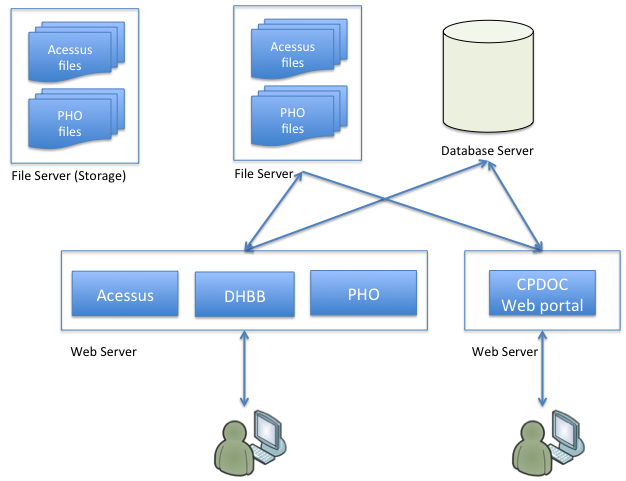
\includegraphics[width=.7\textwidth]{cur-architecture.png}
  \caption{CPDOC's current architecture}\label{fig:cpdoc-today}
\end{figure}

\subsection{Personal Archives (Acessus)}

This system is composed by personal
files from people who influenced the political and social scenario of
our country. These historical documents, in textual or audiovisual form, 
%are precious sources of knowledge that help us to know deeper our history. They may be 
in form of handwritten and printed texts, diaries, letters,
photographs, speeches or memos, represent much more than private
memories: they are the registry of a whole collective memory.

Currently, more than 200 personal archives from
presidents, ministers, military personal and other Brazil's important
public figures compose the CPDOC's collections. Together, they
comprise nearly 1.8 million documents or 5.2 millions pages. From
this, nearly 700 thousands pages are in digital format and the
expectance is to digitize all collections in the next few years. The
collection entries metadata are stored in an information system called
Acessus. It can be accessed through the institution's intranet for
data maintenance or by internet for simple data query.
% that provides and web interface in the FGV's intranet for data query,
% insert, delete and update. The web interface also provides simple
% reports generation interfaces.
Currently, allowed queries are essentially syntactic, i.e.,
% The reports and queries are
restricted to keywords searches linked to specific database fields
defined in an \emph{ad hoc} manner. For those documents that are
already digitized, two digital file versions were generated: one in
high resolution aiming long-term preservation and another in low
resolution for web delivery. High resolution files are stored in a storage system
with disk redundancy and restricted access, while low resolution files
are stored in a file
server~\footnote{\url{https://en.wikipedia.org/wiki/File_server}.}
(Figure~\ref{fig:cpdoc-today}).
% stores the low resolution versions of the digital files
% The files of the already digitalized documents are stored in two
% separated file
% servers~\footnote{\url{https://en.wikipedia.org/wiki/File_server}.}. One
% of them is a storage system with disk redundancy that stores the high
% resolution version of the files for long-term preservation. These
% files are available to a limit number of people with authorized
% access. The second file server stores low resolution versions of the
% digitial files that were used by the web systems and CPDOC's portal
% (Figure~\ref{fig:cpdoc-today}).

\subsection{Oral History Interviews (PHO)}

The CPDOC collection of Oral History hosts currently more than 6.000
hours of recording, corresponding to nearly 2.000 interviews.  More
than 90\% of it, video or audio, are in digital format. For the time being,
two kinds of queries are available in the database: query by subject and
query by interviewed. Each interview record holds a brief technical
information and a summary with descriptions of the interview
themes in the order they appear in the record. Only 10\% of the
interviews are transcribed, and to access the audio/video content the
user is requested to come personally to CPDOC. 

Currently, CPDOC is
analyzing better ways of making this data available online,
considering different aspects such as the best format, use policies,
access control and copyrights.

As in the case of Acessus, the database actually stores only the
metadata about the interviews, while digitized recorded audios and
videos are stored as digital files in the file servers.


\subsection{Brazilian Historical-Biographic Dictionary (DHBB)}

The Brazilian Historical-Biographic Dictionary (DHBB) is certainly one
of the main research sources for contemporary Brazilian politicians
and themes. It contains more than 7.500 entries of biographic and
thematic nature, i.e., people, institutions, organizations and events
records carefully selected using criteria that measure the relevance
of those to the political history for the given period. The entries
are written evenly, avoiding ideological or personal
judgments. CPDOC researchers carefully revise all entries added to
ensure the accuracy of the information and a common style criteria.

%Since it was launched, the DHBB has been an important source of
%information for researches, supporting the drafting of numerous theses
%and dissertations. For instance, Michael Conniff, Director of Global
%Studies Program and Professor of History at San Jose State University
%(California, EUA), after conducting an interesting prosopographical
%study over a selection of biographies extracted from DHBB, could draw
%a profile of the politicians who occupied important positions in the
%government after 1930 \cite{conniff}. Every biographic entry follow a
%common structure of writing that brings all those information beside
%conjunctures of Brazilian history.

The DHBB's database stores few metadata concerning each entry,
and the query is limited to keywords within the title or text.

% \subsection{CPDOC portal and public access interface}

% The three systems presented above share a common relational
% database. The implementation was conceived so as to facilitate the
% construction of a single query interface over all CPDOC archives in
% the CPDOC's web portal. In CPDOC's web portal users are required to
% login in order to access data, and the query interface available in
% there is the only means for reach that.

%%% Local Variables: 
%%% mode: latex
%%% TeX-master: "article"
%%% End: 


\section{Current Status}\label{sec:problems}

In this section we summarize the main problems identified in CPDOC's
current infrastructure and daily working environment.

As described in Section~\ref{sec:cpdoc}, CPDOC's archives are
maintained by three different information systems based on traditional
relational data models. This infrastructure is hard to maintain,
improve and refine, and the information is not found or accessed by
standard search engines for two reasons mainly: (1) an entry page does
not exist until it is created dynamically by an specific query; (2)
users are required to login in order to make queries or access the
digital files. Service providers do not access data directly and
therefore cannot provide specialized services using it. Users
themselves are not able to expand the queries over the collections,
being limited to the available user interfaces in the website.
Thereupon, data of CPDOC's collections is currently limited to what is
called ``Deep Web''~\cite{bergman2001white}.

% The information systems do not provide an intuitive and effective
% interfaces to their users, making the access to information difficult
% and limited.

% The information systems were designed and developed in the 90's and
% since then has undergone several modifications. The changes were
% motivated by different reasons: from requirements of users to
% substitution of obsolete technologies (database systems or web
% development frameworks and programming languages). A careful
% analysis of CPDOC systems would consider them to be outdated
% especially if compared with the current available systems and
% technologies for data storage, indexing and long-term preservation.

The maintenance of current different information systems is very
problematic. It is expensive, time demanding and
ineffective. Improvements are hard to implement and therefore
innovative initiatives are usually postponed. A relational database
system is not easily modified, because relational data models must be
defined \emph{a priori}, i.e., before the data acquisition's
stage. Moreover, changes in the database usually require changes in
system interfaces and reports. The whole workflow is expensive, time
consuming and demands different professionals with different skills
from interface developers to database administrators.

Concerning terminology, CPDOC's collections do not follow any metadata
standards, which hinders considerably the interoperability with other
digital sources. Besides, the available queries usually face
idiosyncratic indexing problems with low rates of recall and
precision. These problems are basically linked to the \emph{ad hoc}
indexing strategy adopted earlier to define database tables and
fields.

% The maintenance of 3 different information systems is expensive,
% time demanding and ineffective. Improvements are hard to implement
% and therefore innovative initiatives are usually postponed. We
% believe this is a side effect of the adoption of a relational data
% model and the traditional information systems maintenance
% methodology.
% % Regarding the items above, it is perhaps worth justifying in
% % technical detail the last one.
% In a relational database system, it is well known that it is
% expensive and hard to frenquently change the data model. This is due
% to the assumption that a relational data model must be defined
% \emph{a priori}, i.e., before the beginning of data
% acquisition. Moreover, information systems for maintenance of
% relational databases are also difficult to evolve. Changes in the
% database require adaptations in the system interfaces and
% reports. This workflow is expensive, time consuming and demands
% several different professionals with different skills: interface
% developers, database administrators etc.

% The CPDOC researchers rely on the FGV's technical staff team from
% the IT department for any database modification or user interface
% improvement. Even the addition of a new field in a table requires a
% whole workflow comprising: (1) the specification of the requirement;
% (2) the costs and time estimation from the technical staff; (3) the
% appropriate authorization; (4) the allocation of a technical
% profissional or team for a period of time considering the other
% FGV's priorities and demands. This workflow usually takes weeks and
% even months.
%
% Whenever distributed and interoperable data maintenance is required,
% the relational data model fails severely. First, it is not easy to
% keep the model and data independent. Second, data exchange is
% hindered by then different storage strategies for datatypes and
% encodes of strings. Third, relational data models are commonly
% flooded with several auxiliary tables necessary to store non-trivial
% relations like N-N relations or generalizations. And finally, in
% general, few model constrains are maintained in databases, and the
% ones created are also not easily interoperable.

% Concerning data storage, it is also worth mentioning that Acessus
% and Oral Historic Interviews collections are not stored in a single
% place. The actual files (digitalized documents) of personal archives
% and the files of digitalized interviews are scattered in different
% file servers.

Finally, data storage is also an issue. Digitized Acessus's documents
and Oral History's interviews are not stored in a single place, but
scattered in different file servers. The CPDOC database only stores
the metadata and file paths to the file servers, making it very
difficult to ensure consistency between files, metadata information
and access control policies.

% Whereas people make great use of standard search engines to query
% and share knowledge, it becomes certainly one of the greatest
% challenges faced by CPDOC when it comes to open their collections.

%%% Local Variables: 
%%% mode: latex
%%% TeX-master: "article"
%%% End: 

\section{The proposal}\label{sec:proposal}

As discussed in Section~\ref{sec:problems}, relational databases are
often hard to maintain and share. Also, the idea of having in-house
developed and closed source information systems is being increasingly
replaced by the concept of open source systems. In such systems the
responsibility of updating and creating new features is not sustained
by a single institution but usually by a whole community that share
knowledge and interests with associates. In this way the system is
kept up-to-date, accessible and growing much faster due to the
increased number of contributors. Such systems are usually compatible
with standards in a way to garantee their widely adoption.

In this context we suggest that CPDOC improves the way their rich
historical data is maintained, stored and shared. Our proposal
privileges open source systems and a lightweight, shared way of
dealing with data. Concretely, we propose the substitution of the
three CPDOC systems by the following technologies.

% It is important to mention that CPDOC has currently three different
% information systems. Althought in the first stage the pilot project
% will involve only the DHBB system, this article is about the whole
% vision of the CPDOC data migration. This system was chosen due to
% different administrative reasons, but also because it has the
% simplest data model.

The Acessus and PHO systems data and files would be stored in an open
source institutional repository software such as
Dspace~\footnote{\url{http://www.dspace.org/}}, Fedora Commons
Framework~\footnote{\url{http://www.fedora-commons.org}} or a more
specialized repository management system like
ICA-AtoM~\cite{van2009ica}~\footnote{\url{https://www.ica-atom.org}}. In
this article we assume the adoption of Dspace with no prejudice of
theoretical modelling. The Acessus data model comprises personal
archives that contains one or more series (which can contain also
other series in a stratified hierarchy) of digitalized documents or
photographies. The PHO system data model is basically a set of
interviews grouped according to some defined criteria within the
context given by funded projects. For instance, a political event
could originate a project which involve interviewing many important
people taking part on the event.

% These projects are the motivation and origin of financial support
% for a series of interviews conducted by CPDOC team with a specific
% purpose.

It is possible to consider that Acessus and PHO systems are basically
responsible for maintaining collections of documents organized in a
hierarchical structure. In this way, one can assume that any digital
repository management system (DRMS) have all required
functionalities. Besides that, DRMS share features desired but not
present in Acessus or PHO, such as: (1) data model based on standard
vocabularies like Dublin Core~\cite{dc} and SKOS~\cite{skos}; (2)
long-term data preservation functionalities (tracking and
notifications of chances in files); (3) fine-grained access control
policies; (4) flexible user interface for basic and advanced queries;
(5) compliance with standard protocols for repositories
synchronization and interoperability (e.g., OAI-PMH~\cite{oai}); (6)
import and export functionalities throuth standard file formats and
protocols; and more.

When it comes to the DHBB system, its relational model is a couple of
tables that store metadata about the dictionary entries (stored in a
single text field of a table). The actual dictionary entries are
created and edited in text editors outside the system and imported to
the system after the whole process of creation and revision. 

% In this way, the system does not maintain the history of
% changes. The content of the entries are saved in HTML~\cite{xhtml}
% format. The HTML is generated by the different text editors used
% making it not uniform, clean or portable and long-term compatible.

The nature of its data suggests that DHBB entries could be easily
maintained as text files using a lightweight human-readble markup
syntax. The files would be organized in a intuitive directory
structure and kept under version control for coordinated and
distributed maintenance. The use of text
files~\footnote{\url{http://en.wikipedia.org/wiki/Text_file}} have a
couple of reasons. They are: easy to maintain using any text editor
(tool independent) allowing the user to choose the best editor for
him; conform to long-term standards by being software and plataform
independent; easy to be kept under version control by any modern
version control
system~\footnote{\url{https://en.wikipedia.org/wiki/Revision_control}.}
since they are comparable (line by line) and efficient at storing
information~\footnote{A text file of a DHBB entry has usually 20\% the
  size of a file DOCX (Microsoft Word) of the same entry.}.

It is interesting to notice that the adoption of a version control
system will allow all file exchanges be recorded and the whole process
be controlled without any need of sophisticated workflow systems,
following the methodology developed by open sources communities for
open source softwares maintenance. For instance,
Git~\footnote{\url{http://git-scm.com}.} is specially developed to
ensure data consistency and keeping track of chances, authorship and
provenance. The use of a version control system will improve the
current workflow of DHBB reviewers and coordinators, since presently
there is no aid system for this task, basically performed using
Microsoft Word text files and emails.

% Most of the suggested technologies are of daily use to most people
% with technical profile, such as software developers, but not very
% familiar to people with non-technical profile. In this context, a
% big challenge of this approach is to motivate the internal users of
% CPDOC systems, i.e., CPDOC archives maintainers, to invest their
% time to learn new technologies, instead of keeping their inefficient
% but known way of dealing with data.

This proposal ideas are already implemented partially for evaluation
purpose only. Figure~\ref{fig:dia-1} illustrates the necessary steps
to full implement our proposal. In the next pagraphs we will briefly
describe each step.

\begin{figure}[htbp]
  \centering
  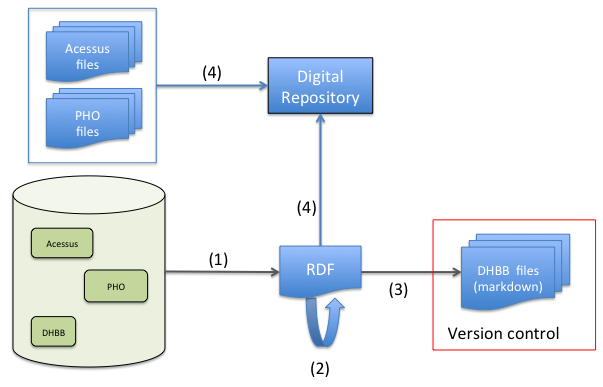
\includegraphics[width=.6\textwidth]{migration.png}
  \caption{Migrating from relational databases to the proposed model}\label{fig:dia-1}
\end{figure}

In step (1) the relational database was exported to
RDF~\cite{rdf-primer} using the open source D2RQ~\cite{d2rq} tool. The
D2RQ mapping language~\cite{d2rq-map} allows the definition of a
detailed mapping from the current relational model to a graph model
based on RDF. The mapping from the relational model to RDF model was
already defined using the standard translation from relational to RDF
model sketched out in \cite{dbANDrdf}. The mapping created so far
defers any model improvement to step (2) described below.

% Until CPDOC team decide about the adoption of the proposed
% technologies and for the abandonment of the current architecture,
% the generated RDF can be updated whenever necessary using D2RQ.

In step (2) we will create a refinement of the graph data model
produced in step (1). The ideia of the refinement is to produce a data
model based on standard vocabularies like Dublin Core~\cite{dc},
SKOS~\cite{skos}, PROV~\cite{prov} and FOAF~\cite{foaf}. The use of
standard vocabularies will make it interchangeable with other models
and facilitate its adoption by service provides and users. In
Section~\ref{sec:model} we describe in more detail the idea of this
refinement. Moreover, this step will also help to better understand
all database model and its semantics.

In step (3) a text file is produced for each DHBB entry. Each text
file holds the entry text and metadata.~\footnote{It is out of the
  scope of this article to present the final format of these files.}
The files use YAML~\cite{yaml} and Markdown~\cite{markdown} markup
languages to describe the metadata and entry content. We choose to
adopt YAML and Markdown because both languages are human-readable
markups for text files and are supported by almost all static site
generators~\footnote{In this application we used Jekyll,
  \url{http://jekyllrb.com}, but any other static site generator could
  be used.}. The use of a static site generator gives to the DHBB
maintainers complete control over the deployment of a DHBB browsable
version.

% Using some scripts that we can easly develop they could deploy a
% DHBB version in three steps: (a) syncronized his repository with the
% repository of other contributors; (b) check the text files to make
% sure that the necessary metadata are presented and have the expected
% values; and (c) compile the files generating a complete website that
% could be made available for the public using a web server and even
% distributed in mirrors servers.

% Actually, each DHBB contributor could generate his one browsable
% DHBB for navigate through the DHBB entries.

Finally, note that step (3) was actally implemented to use the initial
version of the RDF produced in step (1). In the future, the code could
be easly adapted to use the final RDF model produced by step (2).

In step (4) the digital files and their metadata will be imported into
the DRMS. This step will be much easier to be done using the RDF
produced in step (2) than having to access the original database. For
complete this step we only have to decide about the repository
management system that will be adopted, install it in a server and
create the necessary scripts.

% Considering that all DRMS have detailed control access mecanisms, we
% believe that both high and low resolution files can be imported to
% the same digital repository making only the low resolution open for
% public access. This is necessary mainly for preserve bandwidth and
% because in general, the low resolution files also contain some
% watermark and embeded metadadata.

% The migration of the data from relational databases to
% RDF~\cite{rdf} and a simple prototype for browse the data was
% implemented using Jekyll System~\footnote{\url{http://jekyllrb.com}}
% and query support was provided by Apache Solr~\cite{solr} was built
% and used.

The proposed architecture is presented in Figure~\ref{fig:dia-2} and
will be described briefly in what follows. Remember that one of our
main goals is to make the CPDOC archive collections available as open
linked data. Usually, this is accomplished by providing the data in as
RDF/OWL files for download and a SPARQL Endpoint~\cite{sparql} for
queries. Since data and evolve constantly, CPDOC teams would have the
agree on a periodical releases of the data. Besides the RDF/OWL files
and the SPARQL Endpoint, we believe that it is also important to
provide a lightweight and flexible web interface for end users browse
and query the data. This can be easily done using a static website
generator and Apache
Solr~\footnote{\url{http://lucene.apache.org/solr/}} for advanced
queries. Note that the produced website, the RDF/OWL files and SPARQL
Endpoints are complementaries outputs and potencially serve to
different purpose and users. As a modern index solution, Solr can
provide much powerful and fast queries support when compared to
traditional relational database systems. This sum up the ideas of the
architecture.

\begin{figure}[htbp]
  \centering
  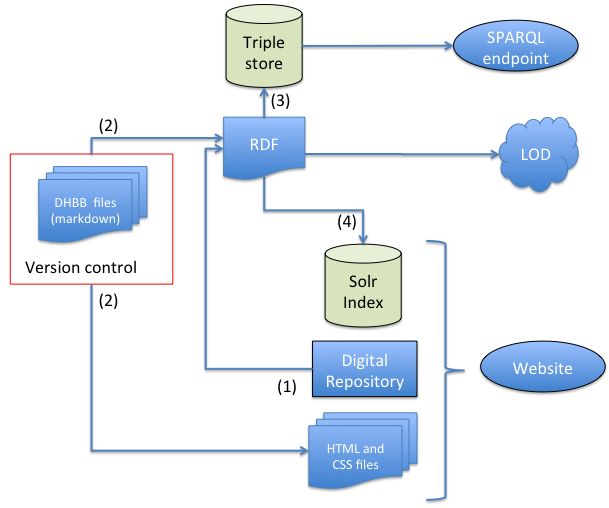
\includegraphics[width=.6\textwidth]{new-architecture.png}
  \caption{The final architecture}\label{fig:dia-2}
\end{figure}

Finally, it is vital to stress the main contrast between the new
architecture and the current one. In the current CPDOC architecture
the data is stored in relational databases and maintained by
information systems. This means that any data modification or
insertion is available in real time for CPDOC website users. However,
this architecture has a lot of drawbacks as mentioned in
Section~\ref{sec:problems}, and also the nature of CPDOC data does not
require continous updates, which means that the cost of this
synchronous \emph{modus operandi} is not needed. Usually, CPDOC teams
work on projects basis and new collections, documents and metadata
revisions are not released so often.

% \section{DHBB: study of case}

% The scope of the proposed implementation is limited, at first, to
% the entries of DHBB. The reason lies in the fact that the data model
% is the simplest of the three and also due to the unconditional
% support received by DHBB managers for our reformulation.  We aim to
% implement a lightweight web interface prototype for browsing and
% querying CPDOC's collections; scripts to produce the RDF file for
% distribution of CPDOC archives releases; scripts to upload the CPDOC
% collections and files into the Dspace system; and a git repository
% for the DHBB files. All these steps are described in this section.

% illustrates the steps of the migration process from the relational
% database to the proposed model. In step (1) the relational database is
% exported to an RDF file using the open source D2RQ~\cite{d2rq}
% tool. The D2RQ mapping language~\cite{d2rq-map} allows the definition
% of a detailed mapping from the current relational model to a graph
% model and implements most of the ideas currently recommended by the
% W3C's R2RML mapping language~\cite{r2rml}.

% The Acessus and PHO collections of documents, images, audio and video
% files will be stored in the DRMS. Users can consult the DRMS directly
% or the collections and items metadata could be exported and integrated
% with additional information (DHBB and complementary data) into the
% final model (one or more RDF files). DHBB editors could generate from
% the YAML+Markdown some RDF files.

% In step (1) a script is used to syncronize the triple store with the
% digital repository metadatas. In step (2) the DHBB files are processed
% to generate the static website... the PHO and Acessus digital
% repository is queried and a RDF file is produced with a dump of its
% current state. The RDF files generated in steps (1) and (2) are
% combined into a single RDF file that is imported to a triple store. In
% (3) the combined RDF file with a snapshot of CPDOC data is made
% available for download or queries through a SPARQL Endpoint provided
% by the Triple Store. In (4) a Solr Instance Index is updated, serving
% as a back-end to a lightweight web interface that provides faced
% search and browsing interfaces of an integrated view of CPDOC
% collections. As a modern web development framework, Solr can provide
% much better and fast queries support when compared to traditional
% relational database systems.

% It is possible to notice that the steps of Figure~\ref{fig:dia-2}
% need not be synchronized, even though CPDOC teams could agree to
% follow a common data release schedule. For instance, if a specific
% release of CPDOC complete archives is planned but the DHBB team was
% not able deliver a new DHBB version in time, new RDF/OWL files
% release can be delivered normally. It would contain the last
% versions delivered by each team, with no prejudice to the others.

The result obtained so far encouraged us to proposed a complete data
model aligned with open linked data vocabularies. In the next section
we will present an outline of how we suggest to do such map.

% FICOU MUITO FORA DE CONTEXTO To make CPDOC data widely used and
% available, we also suggest that CPDOC should define a annual
% schedule for distribution snapshots of its archives in RDF
% format. The RDF file(s) could be offer for download and online
% available for queries in a triple store with a SPARQL endpoint. In
% the next section we further describe the proposal architecture.

% In step (2) scripts use the RDF file produced in the step (1) to
% migrate files and metadata of Acessus and PHO systems to the open
% source repository software DSpace. The mapping of Acessus data to
% Dspace is described in Table~\ref{tab:map}. The mapping of PHO
% interviews is basically consisted of linking each project to a
% collection and each interview to an item with the respectively
% bitstreams (digital audio or video files).

% \begin{table}[htbp]
% \centering
% \begin{tabular}{rcl}
% Acessus &  & Dspace \\ \hline
% personal archives & $\to$ & communities \\
% series & $\to$ & collections \\
% documents or photographies metadata & $\to$ & items \\ 
% documents or photographies files & $\to$ & bitstreams \\ \hline
% \end{tabular}
% \caption{Mapping from Acessus to Dspace}\label{tab:map}
% \end{table}

% In step (3) the RDF model created is improved based on linked data
% concepts, i.e., considering the adoption of standard vocabularies and
% ontologies such as FOAF~\cite{foaf}, SKOS~\cite{skos}, Dublin
% Core~\cite{dc} and PROV~\cite{prov}. This refined RDF file would be
% available in form of periodic releases of CPDOC's collections that
% would be much more interoperable and useful for service providers.

% In step (4) Markdown~\cite{markdown} files are created using
% YAML~\cite{yaml} metadata header for each DHBB entry. YAML is a
% lightweight markup language for metadata description in a
% human-readable text file, while Markdown allows people to write text
% using an easy-to-read, easy-to-write plain text format that can be
% converted to structurally valid XHTML~\cite{xhtml} (for online use) or
% PDF (for printing). These files can be host in a distributed
% versioning control environment for collaborative maintenance. This can
% be achieved using Git~\cite{git}, a distributed version control system
% which is suitable for many different models of collaborations.

% Some tools are available for this kind of conversion and one of the
% most established is the D2RQ~\cite{d2rq}. Once the RDF is generated,
% several steps for improving and enriching the RDF file, checking for
% data consistency and gathering new data connections using the
% available knowledge sources (ontologies, dictionaries etc) is
% planned.  This environment of a group of files organized in a
% directory structure under control of a version control system and
% the RDF interface is meant to compose the new data storage for DHBB.

% Figure~\ref{fig:dhbb-ex} shows a fragment of a YAML+Mardown file from
% a DHBB entry, just as an example. Lines 1--16 are the YAML header with
% the metadata about the entry. The entry content is written in Markdown
% as observed from the line 17 on. In Line 18 it is possible to see that
% references to metadata fields can be made inside the body of the entry
% written in Markdown.

% \begin{figure}[thbp]
%   \centering
% \begin{lstlisting}[frame=single,numbers=left,basicstyle=\footnotesize\ttfamily]
% ---
% type: biliography
% created-by: 2010-03-04T17:55:58,83Z
% title: Assad Junir, Mario
% reviewer: Fulano
% author: Beltrano
% positions: 
%  - dep. fed. MG 1998-1999
%  - dep. fed. MG 2000-2002
%  - dep. fed. MG 2003-2007
% sources: 
%  - Camara dos Deputados; DIAP (Ago./06); Diario de Sao Paulo
%    (online) 29/10/2003. at http://oglobo.globo.com/diariosp.
%  - Portal Caparao (online) 01/jun/2007 e 15/maio/2008. Disp.
%    em http://www.portalcaparao.com.br.
% ---

% {{ title }}

% *Mario Assad Junior* nasceu em Manhuacu (MG) no dia 11 de 
% agosto de 1965, filho de [Mario Assad](/dhbb/mario-assad.html) 
% e de Nedi Vieira Assad. Seu pai foi deputado estadual em Minas 
% Gerais de 1967 a 1975 e de 1978 a 1983, secretario do Trabalho, 
% Acao Social  e Desporto de 1975 a 1978, deputado federal de 
% 1983 a 1991, secretario de Justica de 1991 a 1994 e prefeito 
% de Manhuacu entre 2001 e 2004.
% ...
% \end{lstlisting}
% \caption{YAML+Markdown file of a DHBB entry}\label{fig:dhbb-ex}
% \end{figure}

% Figure~\ref{fig:dia-2} shows how the CPDOC data is supposed to be
% maintained in our model. In step (1) a script is used to generate the
% current DHBB repositoty state RDF file for a DHBB maintainer. In step
% (2) the PHO and Acessus digital repository is queried and a RDF file
% is produced with a dump of its current state. The RDF files generated
% in steps (1) and (2) are combined into a single RDF file that is
% imported to a triple store. In (3) the combined RDF file with a
% snapshot of CPDOC data is made available for download or queries
% through a SPARQL Endpoint provided by the Triple Store. In (4) a Solr
% Instance Index is updated, serving as a back-end to a lightweight web
% interface that provides faced search and browsing interfaces of an
% integrated view of CPDOC collections. As a modern web development
% framework, Solr can provide much better and fast queries support when
% compared to traditional relational database systems.

% \begin{figure}[thbp]
%   \centering
%   \includegraphics[width=.9\textwidth]{diagrama2.png}
%   \caption{Data maintainance}\label{fig:dia-2}
% \end{figure}

% It is possible to notice that steps (1) and (2) of
% Figure~\ref{fig:dia-2} need not be synchronized, even though CPDOC
% teams could agree to follow a common data release schedule. For
% instance, if a specific release of CPDOC complete archives is planned
% but the DHBB team was not able deliver their version in time, the
% release can be delivered normally. It would contain the last versions
% delivered by each team, with no prejudice to the others.

%%% Local Variables: 
%%% mode: latex
%%% TeX-master: "article"
%%% End: 


\section{Improving Semantics}\label{sec:mapping}

More than improving the current infrastructure for storing and
accessing CPDOC data, we would like to exploit the semantic
possibilities of such rich source of knowledge. One of the ways to do
that is to embed knowledge from other sources by creating links within
the available data. Since much of the data is related to people and
resources with historical relevance, or historical events, some
available ontologies and vocabularies can be used in this task.

The personal nature of the data allows us to use projects that are
already well developed for describing relationships and bonds between
people, such as FOAF~\cite{foaf} (Friend of a Friend) -- a vocabulary
which uses RDF to describe relationships between people and other
people or things. FOAF permits intelligent agents to make sense of the
thousands of connections people have with each other, their belongings
and historical positions during life. This improves accessibility and
generates more knowledge from the available data.

The analysis of structured data can automatically extract connections
and, ultimately, knowledge. A good example is the use of
PROV~\cite{prov}, which provides a vocabulary to interchange
provenance information. This is interesting to gather information of
data that can be structurally hidden in tables or tuples.
% For instance [EXAMPLE].

The RDF graph model enables also the merging of data content
naturally. The DBpedia project, for instance, allows users to query
relationships and properties associated with Wikipedia resources, and
users can link other datasets to the DBpedia dataset in order to
create a big and linked knowledge knowledge base. CPDOC could link
their data to DBpedia and then make their own data available for a
bigger audience.
% The DBpedia project, for instance, provide URIs~\footnote{Uniform
% resource identifier,
% \url{https://en.wikipedia.org/wiki/Uniform_resource_identifier}.}
% which enable the connection of these resources with different
% sources of data in order to create a big and linked knowledge
% database.  CPDOC can use DBpedia to link their data to already
% available resources in DBpedia making their own data available to a
% bigger audience.

In the same direction, the use of lexical databases, such as the
WordNet~\cite{wordnet} and its Brazilian version
OpenWordnet-PT~\cite{wordnet-br}, will allow us to make natural
language processing of DHBB entries. Named entities recognition and
other NLP tasks can automatically create connections that improve
dramatically the usability of the content.
% The Brazilian OpenWordnet-PT provides a lexical resource for
% Portuguese complete mapped to the original english WordNet.
Other resources like YAGO~\cite{yago} and BabelNet~\cite{babelnet}
links Wikipedia to WordNet. The result is an ``encyclopedic
dictionary'' that provides concepts and named entities lexicalized in
many languages and connected with large amounts of semantic
relations. Finally, the SUMO Ontology~\cite{sumo} could also be used
to provide a complete formal definition of terms linked to
WordNet. All of these lexical resources and ontologies will be further
explored when we start the natural language processing of DHBB
entries.

% Much of the effort proposed is related to integrating the data
% available to other sources of knowledge, improving both
% accessibility and usability of the data CPDOC holds. To do so, it is
% imperative to migrate the current CPDOC database model to a open,
% shared and modern one, aligned with semantic web directives,
% ontologies and vocabularies. This improvement is highlighted is what
% we called the refinement of the RDF model when we described
% Figure~\ref{fig:dia-1}.  It what follows, let us give an example of
% the proposal refinement considering a fragment of the original CPDOC
% relational model.

\begin{figure}[htbp]
  \centering
  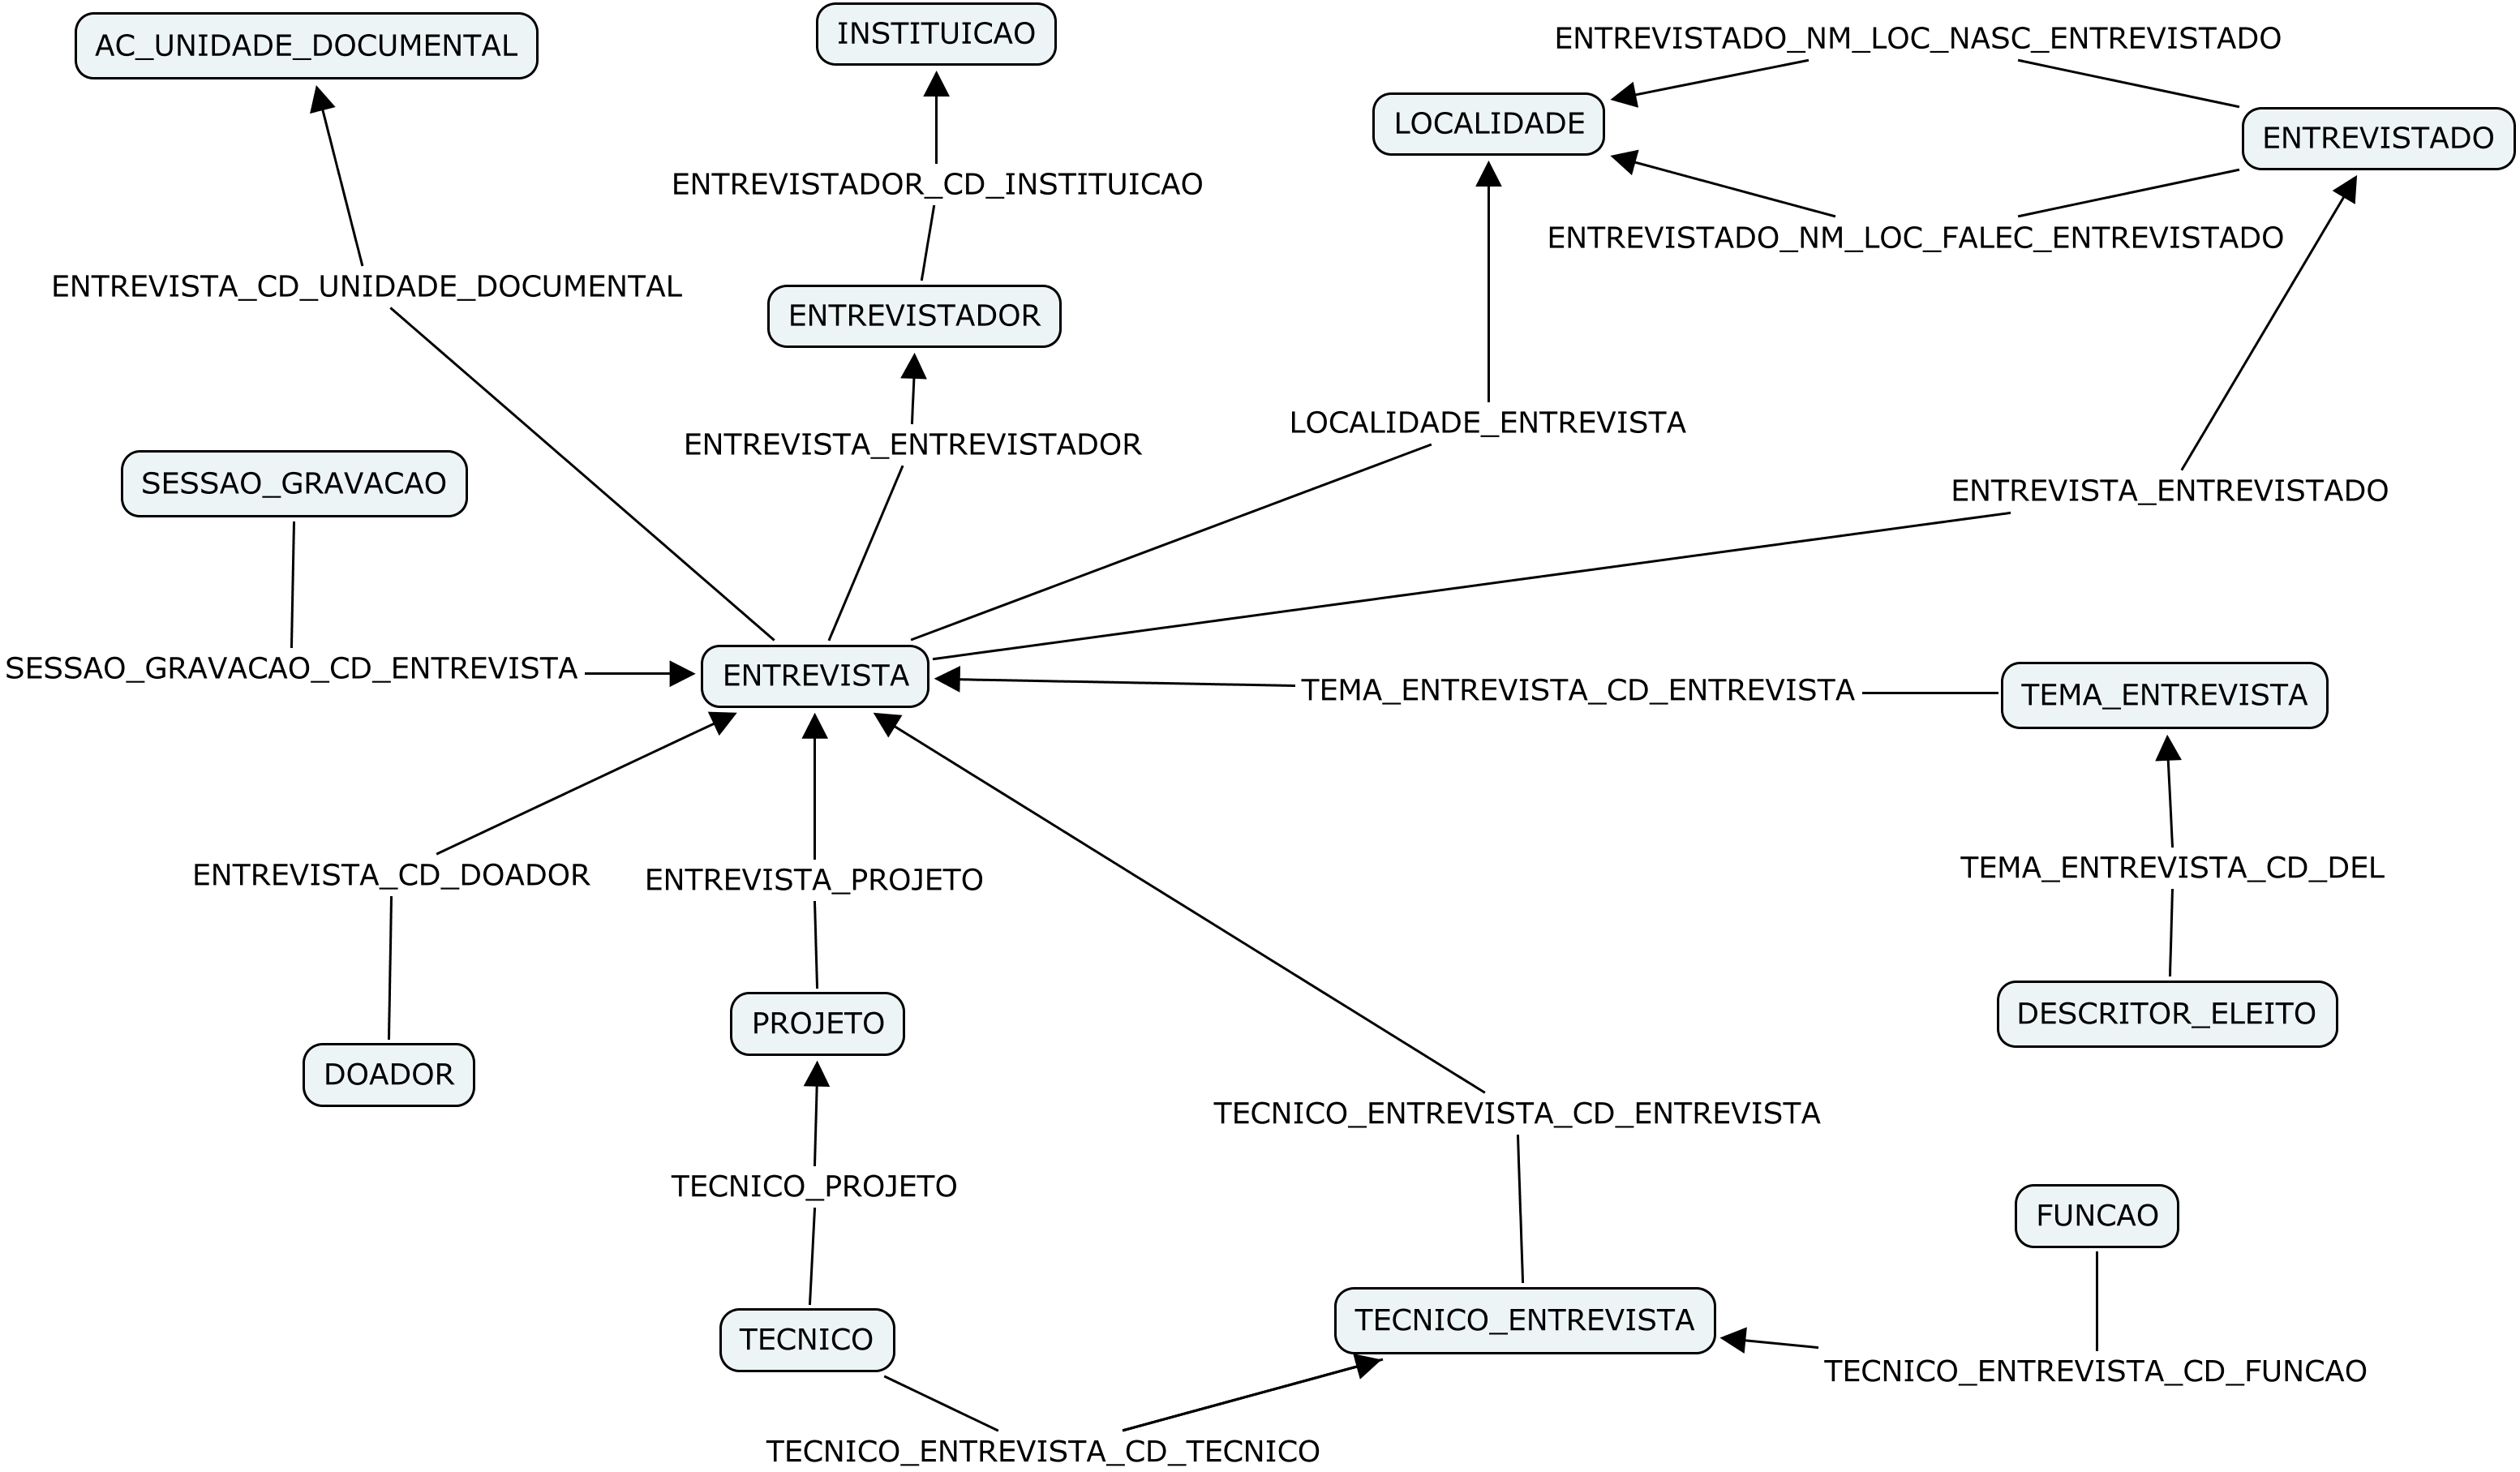
\includegraphics[width=.8\textwidth]{pho.png}
  \caption{PHO first RDF model}\label{fig:pho}
\end{figure}

% What is important to note in the model presented in
% Figure~\ref{fig:pho} is that besides simple translations from
% relational to graph model, D2RQ was not able to automatic improve
% much further the model. Let us highlight some cases. D2RQ was able
% to correctly translate relations N:M in the relational model, such
% as \texttt{entrevista\_entrevistador} (originally a table in the
% relational model) to a property that connect directly instances of
% \texttt{entrevista} (Interview) with instances of
% \texttt{entrevistador} (Interviewer). Nevertheless, the N:M relation
% between \texttt{entrevista} and \texttt{tecnico} (technician) was
% kept as a a intermediary class called \texttt{tecnico\_entrevista}
% because of the existence of an aditional information in this N:M
% relation, the role (\texttt{funcao} class) of the technician in the
% interview. More on roles, the relational model also expose some
% inconsistences. Althought connection of the technician and the
% interview is parameterize by its role, the donator, interviewer and
% the interviewee of the interview are modelled each one by a specific
% table. The main problem with this model is that interviewee,
% interviewer, donator and technician are all people with share a lot
% of common properties like name, address and so on. These problems
% are all result of a ``ad hoc'' modeling process. The model, as is,
% only makes sense for CPDDOC team and it could hardly be useful
% outside CPDOC.

Figure~\ref{fig:pho} shows a fragment of the current RDF model
produced by D2RQ (in step (1) of Figure~\ref{fig:dia-1}) using the
original CPDOC database relational model. This fragment shows only
some PHO classes (derived from the tables) and some properties
(derived from the foreign keys). Classes are written inside the boxes
and properties are represented by the names in arrows that connect
boxes.

The model presented in Figure~\ref{fig:pho} depicts that D2RQ was not
able to automatically improve much further the model. D2RQ was able to
correctly translate relations N:M in the relational model, such as
\texttt{entrevista\_entrevistador} (originally a table in the
relational model) to a property that connect directly instances of
\texttt{entrevista} (interview) with instances of
\texttt{entrevistador} (interviewer). Nevertheless, the N:M relation
between \texttt{entrevista} and \texttt{tecnico} (technician) was kept
as an intermediary class called \texttt{tecnico\_entrevista} due to
the existence of an aditional information in this N:M relation, the
role (\texttt{funcao} class) of the interview technician. The
relational model also seems to have some inconsistences. Although the
connection of technician and interview is parameterized by different
roles, the donator, interviewer and interviewed of an interview are
modeled each one in a specific table. In this case interviewed,
interviewer, donator and technician are all people that share a lot of
common properties like name, address, etc, and could be modeled as
people. These problems are all result of a ``ad hoc'' modeling
process. The model defined this way only makes sense for CPDDOC team
and it could hardly be useful outside CPDOC.

\begin{figure}[htbp]
  \centering
  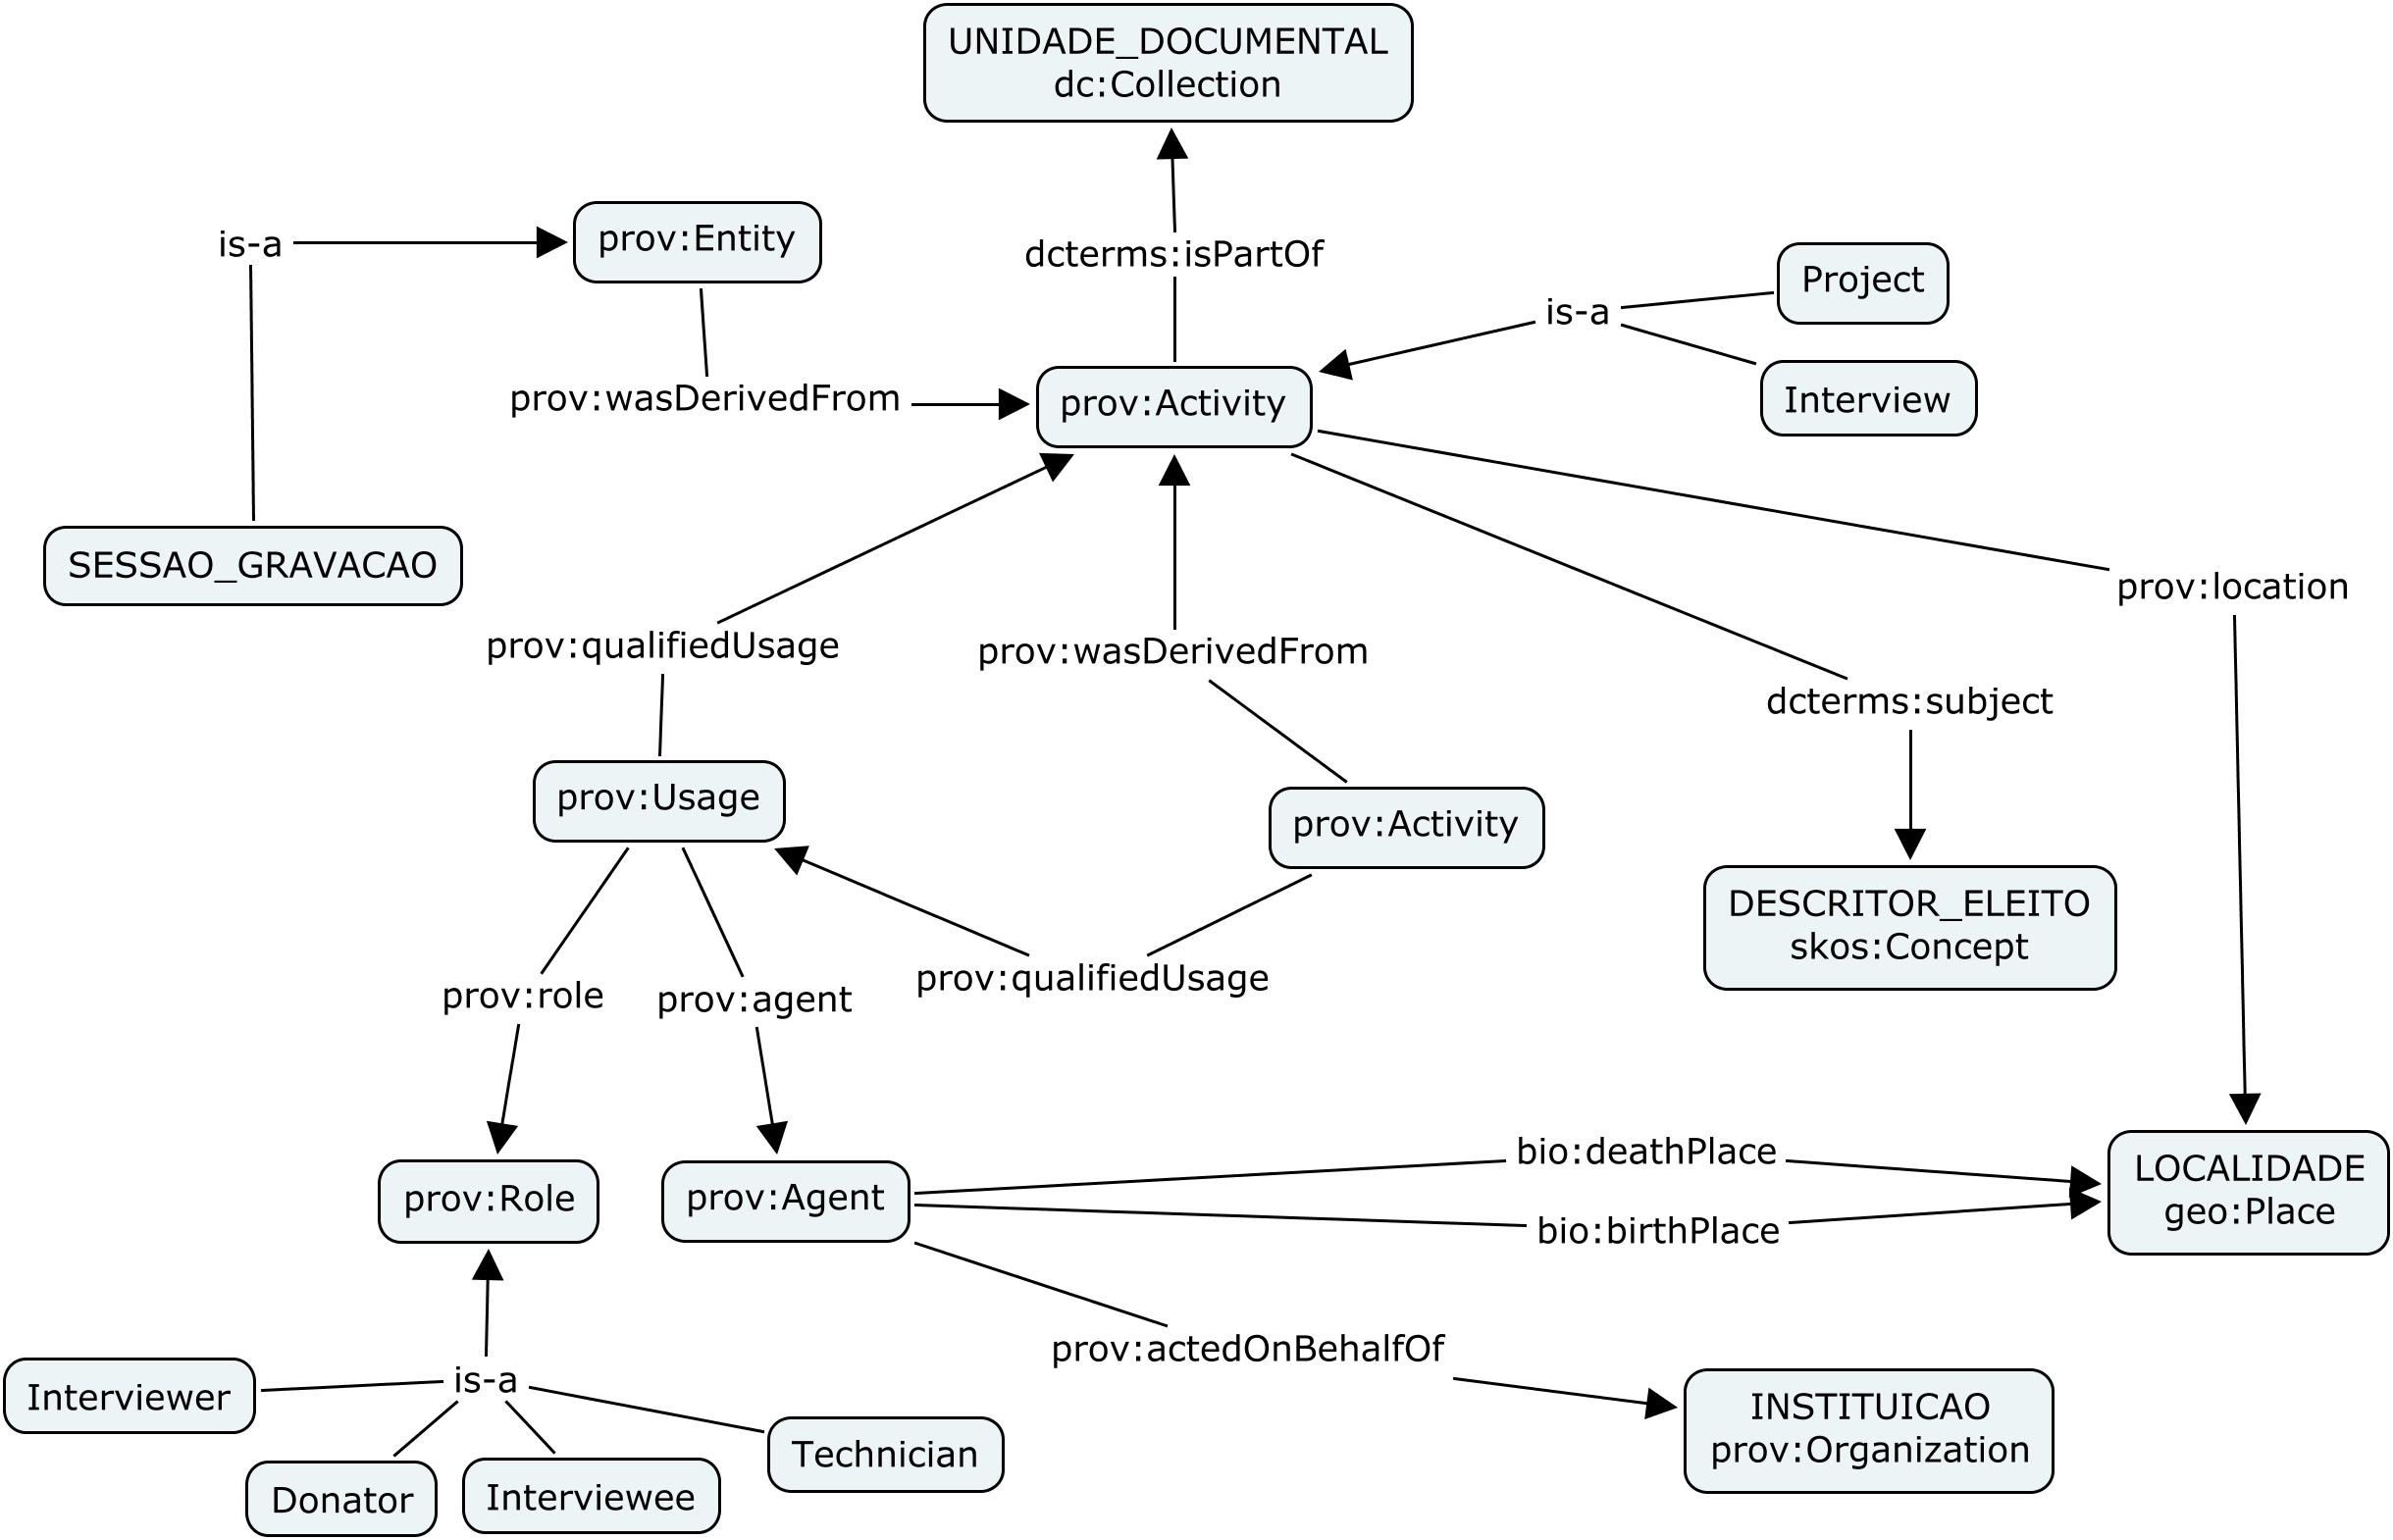
\includegraphics[width=.8\textwidth]{pho-new.png}
  \caption{PHO revised RDF model}\label{fig:pho-new}
\end{figure}

Figure~\ref{fig:pho-new} shows how PHO model can be refined. The new
model uses standard vocabularies and ontologies, making the whole
model much more understandable and interoperable. In the
Figure~\ref{fig:pho-new}, \texttt{prov:Activity} was duplicated only
for a better representation. The prefixes in the names indicate the
vocabularies and ontologies used: \texttt{prov}, \texttt{skos},
\texttt{dcterms}, \texttt{dc}, \texttt{geo}, and \texttt{bio}. We also
defined a CPDOC ontology that declares its own classes and specific
ontology links, such as the one that states that a \texttt{foaf:Agent}
is a \texttt{prov:Agent}. In this model, we see that some classes can
be subclasses of standard classes (e.g. \texttt{Interview}), while
some classes can be replaced by standard classes
(e.g. \texttt{LOCALIDADE}).

%%% Local Variables: 
%%% mode: latex
%%% TeX-master: "article"
%%% End: 


% The new database system composed by Markdown files and periodic RDF
% releases can be easily used for accessing data in an efficient
% way. The figure below illustrates the process. CPDOC and their
% collaborators would be responsible for creating Markdown files that
% would be automatically analyzed by a script for generating the RDF
% file, which would be refined and improved. This refined RDF would be
% made available to the web as linked open data, which would allow the
% information to be accessed and improved by the community. On the other
% hand, the RDF would also be stored in a triple store that allows for
% queries using many different GUI configurations (for instance using
% Solr) to easy the access of data stored. This schema follows a modern,
% open and scalable way of sharing and improving the data stored in
% CPDOC.

\section{Conclusion}

In this paper we presented a new architecture for CPDOC archives
creation and maintenance. The architecture targeted is based on open
linked data concepts and open source methodologies and tools. We
believe that despite the fact that CPDOC users would need to be
trained to use the proposed tools such as text editors, version
control softwares and command line scripts; this architecture would
give more control and easiness for data maintenance. Moreover, the
architecture allows knowledge to be easily incorporated to collections
data without the dependency of database refactoring. This means that
CPDOC team will be much less dependent from FGV's Information
Management and Software Development Staff.

% NÃO SEI SE VALE A PENA FLOREAR A CONCLUSÃO. CORTE, SE ESTIVER
% DEMAIS!  Por fim, entendemos que as possibilidades abertas nesse
% cenário transcendem em muito os limites do mundo digital e
% repercutem diretamente na nossa própria história em construção, na
% maneira como queremos colaborar para a mediação do saber. O ato de
% conhecer não se reduz a uma apreensão inerte de dados, ou tão
% somente advém de apreciações meramente lógicas. As pessoas conjugam
% faculdades cognitivas e perceptivas quando interagem entre si e com
% os recursos que as cercam, participando da construção do
% conhecimento sobre a realidade. O ambiente digital e de rede traz
% infinitas oportunidades de compartilhamento dessa história em
% construção, com desdobramentos na cultura e no aprendizado. Mas para
% que esse ambiente seja efetivamente transformador, é fundamental o
% papel das políticas de difusão e disponibilização dos registros
% históricos, bem como a busca pela sua melhor forma de acesso,
% garantindo a diversidade da qual não podem prescindir.

%Finally, we believe that the possibilities offered by our proposed
%architecture far transcend the limits of the digital world and
%directly affect our own \textit{history in the making}, the way we
%collaborate for the mediation of knowledge. The act of knowing is not
%reduced to an inert seizure of data, nor it comes from assessments
%merely logical. People combine cognitive and perceptual faculties as
%they interact with the resources that surround them, participating in
%the construction of the knowledge over the reality. The digital
%environment and network brings endless opportunities for sharing this
%history in the making, with developments in culture and learning. But
%for this environment to be effectively transformer, is crucial the
%role of policy dissemination and availability of historical records,
%as well as the search for the right way to access it, ensuring the
%diversity which can not do without.

Many proposals of research concerning the use of lexical resources for
reasoning in Portuguese using the data available in CPDOC are being
carried out so as to improve the structure and quality of the DHBB
entries. Moreover, the automatic extension of the mapping proposed in
Section~\ref{sec:mapping} can also be defined following ideas of
\cite{onto-context}. Due the lack of space, we did not present in this
paper.

\bibliographystyle{plain}
\bibliography{sda}

\end{document}


